%                                             -*- coding: utf-8 -*-
% Mindenkinek csak javasolni tudjuk, hogy latex-et használjon.
% Szakdolgozatnál vagy diplománál már egyértelműen kijönnek az
% előnyei a Worddel szemben.  Ennek ellenére ez a sablon messze nem
% tökéletes.  Ha valamit javítanál benne, kérlek, küld vissza, hogy
% hallgatótársaid is profitáljanak belőle.  Köszönöm.

% További nehézséget okoz, hogy a népszerű latex disztribúciók nem
% tartalmazzák a legújabb változatát a magyar.ldf-nek.  A szükséges
% fájlokat a sablon mellé bemásoltuk, de le is tölthetőek innen:
% http://www.math.bme.hu/latex/
%
%
%
\documentclass[a4paper,oneside]{article}
\usepackage[margin=3cm]{geometry}
% =================================================================
% Magyar nyelvi támogatás
%------------------------
% ###################
% Nyelvváltó parancsok:
%\selectlanguage{english}
%\selectlanguage{magyar}
% rövid angol beszúrás:  \foreignlanguage{english}{some english text}
% határozott névelők generálása ``magyar'' babel-el:
% argumentum+megfelelő határozott nevelő: \az{},\Az{}
% csak a megfelelő határozott nevelő: \az*{}, \Az*{}
% címkék: \aref{}, \aref*{}, képletekhez \aref()
%        \Aref{}, \Aref*{}, képletekhez \Aref()
% oldalak: \apageref{}, \apageref*{}
%        \Apageref{}, \Apageref*{}
% idézetek: \acite, \acite*, \Acite, \Acite*
% ###################
\usepackage[english,magyar]{babel} %vegyes nyelvi támogatás a
% magyar helyesírás ellenőrzéshez (ispell) és elválasztáshoz
\selectlanguage{magyar}

%=================================================================
% direkt ékezetes karakter beírás támogatás
%-------------------------------------------
\usepackage[T1]{fontenc}
\usepackage[utf8]{inputenc}
\usepackage{multirow} 
%================================================================
% Undorító dolog bitmappelt (Type III) betűtípust nézni a PDF-ben
% képernyőn. Az alapértelmezett Computer Modern font LaTex-ben
% bitmappelt, ezért használjunk Times fontot:
\usepackage{times}

%================================================================
% ha ábrát akarunk beemelni, akkor használjuk a graphicx/graphics
% csomagot és az \includegraphics[width=<width>]{abra.pdf} parancsot
\usepackage{graphicx} %for graphics
%kepek helye a gyokerhez(ehhez a file-hoz kepest) kepest
\graphicspath{{./figs/}}

%================================================================
% Kötelezően használjuk a hyperref csomagot, mert ezzel többek között 
%  kultúrált hyperlinkelt PDF-et lehet csinálni az alábbi
%  variációkban, különféle hyperref backend-ekkel:
%  pdflatex,dvipdfm,ps2pdf
% tapsztalataim szerint a MikTeX (Win32) a 'dvipdfm' konverzióval
% optimális  míg a teTeX (Linux/Solaris) jobb szereti a 'dvips' módszert
%------------------------------------
% pontosan egyet kommentezzünk be!!!!!!!
% értelemszerűen backend függően generáljunk dvi-ból PDF-et!!!
%------------------------------------
% A hyperref csomag az utolsó beolvasott csomag legyen, kivéve néhány
% problémás csomagot, pl. algorithm
%-----------
% ########################### FONTOS ###########################
% A hyperref hibásan működik a babel csomag 'magyar.ldf' fájljának
% 1.5-ös verziójánál korábbi változatával. 2004. februárjában a MikTeX
% és teTex disztribúciók még csak a v.1.4 verziót tartalmazták! A fájl
% aktuális verziója a BME Matematikai intézet LaTeX honlapjáról
% elérhető: http://www.math.bme.hu/latex/ 
% A lusták kedvéért a jelen sablon mellé is mellékelem:
% magyarlatex_0.01-2.tar.gz 
% ########################### FONTOS ###########################
%-----------
\usepackage[colorlinks=true]{hyperref}

%%%%%%%%%%%%%%%%%%%%%%%%%%%%%%%%%%%%%%%%%%%%%%%%%%%%%%%%%%%%%%%%%%%
% Itt kezdődik maga a dokumentum
%%%%%%%%%%%%%%%%%%%%%%%%%%%%%%%%%%%%%%%%%%%%%%%%%%%%%%%%%%%%%%%%%%
\begin{document}
%%%%%%%%%%%%%%%%%%%%%%%%%%%%%%%%%%%%%%%%%%%%%%%%%%%%%%%%%%%%%%%%%%%
% Ezt ne piszkáld!!!!
%%%%%%%%%%%%%%%%%%%%%%%%%%%%%%%%%%%%%%%%%%%%%%%%%%%%%%%%%%%%%%%%%%%
\pagestyle{myheadings} % legyen fejléc 

\newcommand{\onlabcim}{
  \begin{center}
    \huge{\textbf{Önálló laboratórium beszámoló}}

    \small{Távközlési és Médiainformatikai Tanszék}
  \end{center}
} 

% Argumentumok: #1=Név, #2=Neptunkód, #3=szakirány, #4=email, #5 konzulens-1, #6 konzulens-1-email, #7 konzulens-2, #8 konzulens-2-email
\newcommand{\onlabszerzo}[8]{

\begin{center}
  \begin{tabular}{ r l }
  készítette: & \textbf{#1}  \\
              & \href{mailto:#4}{\textbf{#4}}  \\
  neptun-kód: & \textbf{\texttt{#2}}  \\
  ágazat:     & \textbf{#3}  \\
  konzulens: & \textbf{#5}  \\
             & \href{mailto:#6}{\textbf{#6}} \\
  konzulens: & \textbf{#7}  \\
             & \href{mailto:#8}{\textbf{#8}}  \\
  
  \end{tabular}
\end{center}

}

% % Argumentumok: #1=Név, #2=email
% \newcommand{\konzulens}[2]{
%   \noindent\textbf{Konzulens:} #1 
%   \newline\emph{Email cím:}\/ \href{mailto:#2}{#2}
%   \newline
% 
% }

% Argumentumok: #1=Tanév (xxxx/xx alakban, #2=félév (pont nélkül)
\newcommand{\tanevfelev}[2]{
  \large\noindent\textbf{Tanév:} #1. tanév, #2. félév
  \newline
}

% Argumentumok: #1=téma címe 
\newcommand{\feladatcim}[1]{
  \large\noindent\textbf{#1}
  \bigskip
}

% Argumentumok: #1=téma részletei 
\newcommand{\feladatmaga}[1]{
\large\noindent\textbf{Feladat:} 
  \newline
 #1
 \newline
 \smallskip
}

% A fejezetek közé beágyazott irod.jegyzék
\def\thebibliography#1{\renewcommand{%
\baselinestretch}{1}\subsection{A tanulm\'anyozott irodalom jegyz\'eke}\list
 {\small [\arabic{enumi}]}{\settowidth\labelwidth{[#1]}\leftmargin\labelwidth
 \advance\leftmargin\labelsep
 \usecounter{enumi}}
 \def\newblock{\small \hskip .11em plus .33em minus .07em}
 \sloppy\clubpenalty4000\widowpenalty4000
 \sfcode`\.=1000\relax}
\let\endthebibliography=\endlist%


%%% Local Variables: 
%%% mode: latex
%%% TeX-master: "template"
%%% End: 
 % Ez kell!!!
\markright{Schweitzer András Attila (TLEIB5)} % egyoldalas fejléc!!!
%--------------------------------------------------------------------
% fedlap
%--------------------------------------------------------------------
\begin{titlepage}
%bme logo 
 \begin{figure}[h]
    \centering
      
\includegraphics[width=12cm]{bme_logo}
  \label{fig:bme_logo}
  \end{figure}
  \thispagestyle{empty}
  %cím generálás
  \onlabcim

% \begin{center}
%   \begin{tabular}{ p{3cm} p{5cm} }
%   
%   Készítette: & Schweitzer András Attila  \\
%   Neptun-kód: & TLEIB5  \\
%   Ágazat: & Intelligens hálózatok  \\
%   E-mail cím: & schweitzeraa16@gmail.com  \\
%   Konzulens: & Németh Felicián  \\
%   E-mail cím: & nemethf@tmit.bme.hu  \\
%   Konzulens: & Lévai Tamás  \\
%   E-mail cím: & levait@tmit.bme.hu  \\
%   
%   \end{tabular}
% \end{center}

 
  %\szerzo argumentumok: #1=Név, #2=Neptunkód, #3=szakirány, #4=email,#5 konzulens-1, #6 konzulens-1-email, #7 konzulens-2, #8 konzulens-2-email
  \onlabszerzo{Schweitzer András Attila}{TLEIB5}{Intelligens hálózatok}{schweitzeraa16@gmail.com}{Németh Felicián}{nemethf@tmit.bme.hu}{Lévai Tamás}{levait@tmit.bme.hu}
 
 
%\feladatcim argumentuma a feladat rövid, 1 soros címe
  \feladatcim{Többutas adatátvitel Media over QUIC rendszerben (Media over Multipath QUIC)} 

  %\feladatmaga argumentuma a feladat 1-2 bekezdésnyi ismertetése
  \feladatmaga{
A Media over QUIC (MoQ) egy új, még fejlesztés alatt álló protokollcsalád, 
amelyet internetes médiaadatok hatékony továbbítására terveztek. Ennek egyik 
meglévő megvalósítása a LibQuicR nevű könyvtár, amely jelen feladat alapját képezi.

A feladat célja a LibQuicR módosítása úgy, hogy képes legyen kihasználni a több 
útvonalon történő párhuzamos adatátvitelt (multipath), amit a PicoQUIC nevű, QUIC 
protokollt megvalósító könyvtár biztosít. Ennek érdekében a LibQuicR transzport rétegét 
úgy kell átalakítani, hogy egyetlen kapcsolat keretében több hálózati útvonalat is 
tudjon létrehozni és kezelni a PicoQUIC multipath képességein keresztül.

A módosítások működését egy demonstrációval igazoljuk, amelyet egy virtuális 
tesztkörnyezetben hajtunk végre. Ebben a környezetben több hálózati interfésszel 
rendelkező kliensek vesznek részt, és az adatátvitel során aktívan kihasználjuk 
a multipath lehetőségeket. A teszt során szándékosan megszakítunk egy éppen használt 
útvonalat, hogy bemutassuk: a LibQuicR – az új multipath támogatással – képes 
automatikusan fenntartani az adatfolyam továbbítását, minimális késleltetéssel 
és megszakítás nélkül.}

 
  %\tanevfelev argumentumok:
  % #1=Tanév (xxxx/xx alakban), #2=félév (pont nélkül!)
  
  \tanevfelev{2024/25}{II}
 
\end{titlepage} 

%==================================================================
\section{A laboratóriumi munka környezetének ismertetése,
     a munka előzményei és kiindulási állapota}
\label{sec:kornyezet}
% A munka  előzményei és kiindulási állapota
% \newpage
\subsection{Bevezető}
\label{sec:bevezeto}
%--------------------------------------------------------------------
Napjainkban az internetes adatforgalom túlnyomó részét különféle médiatartalmak – 
elsősorban videók és élő közvetítések – teszik ki. Egyes kutatások 
szerint az internetes forgalom 65\%-a ilyen típusú tartalom lehet \cite{live_stats}. 
Ezek hatékony és megbízható továbbítása azonban komoly 
technológiai kihívást jelent, különösen akkor, ha a felhasználói élményt is 
figyelembe vesszük: az alacsony késleltetés, a megszakításmentes lejátszás 
és a biztonságos adatátvitel alapvető elvárások.

E kihívásokra jött létre válaszként a QUIC protokoll\cite{quic}, amely UDP-alapú, alacsony 
késleltetésű, titkosított és megbízható adatátvitelt tesz lehetővé. Erre épülve 
fejlődik jelenleg a Media over QUIC (MoQ) szabvány\cite{moq_draft}, amely kifejezetten 
médiatartalmak hatékony továbbítását célozza a QUIC képességeit kihasználva.

Ezzel párhuzamosan a felhasználói eszközök – különösen a mobiltelefonok és 
laptopok – egyre gyakrabban rendelkeznek több hálózati interfésszel (például Wi-Fi és 5G). 
Mégis gyakran tapasztalható kapcsolat megszakadás, hosszú töltési idők vagy éppenséggel 
elérhetetlenné váló szolgáltatások, ha az egyik kapcsolat megszakad vagy instabillá 
válik. A többutas adatátvitel lehetőséget kínál ezen problémák áthidalására azáltal, 
hogy párhuzamosan több hálózati útvonalat használ az adatok továbbítására, növelve 
ezzel a robusztusságot és az elérhető sávszélességet.

A jelen munka célja ezen két technológia – egy adott MoQ implementáció és a multipath kommunikáció 
– egyesítése. A cél egy olyan rendszer bemutatása, 
amely képes több útvonalat kihasználva, élő adatfolyamot hatékonyan és megbízhatóan 
továbbítani. Ez nemcsak a hálózati erőforrások jobb kihasználását segíti elő, hanem 
hozzájárul a végfelhasználói élmény javításához is.

%--------------------------------------------------------------------

%<Mit kell tudni a feladatról, esetleges elméleti bevezető (nagyon értelemszerű dolgokat ne 
%definiáljunk, de jó, ha egy kicsit kontextusba kerül a témakör, miért fontos ez nekünk, 
%mi volt eddig, milyen megoldások jöhetnek szóba és miért emellett döntöttünk, milyen kari 
%nagyobb projektbe kapcsolódik ez), stb. Terjedelem max. 50\% beszámolónak.>
%Ennek a résznek az a szerepe, hogy az olvasó számára megmutassa az elvégzett munka tágabb környezetét.>

\subsection{Elméleti összefoglaló}

\subsubsection{A QUIC protokoll}
\paragraph{}
Az internetes multimédia átviteli technológiai fejlődése során egyre 
nagyobb igény mutatkozik olyan protokollokra, amelyek képesek 
rugalmasan és hatékonyan kezelni a valós idejű adatfolyamokat, még 
változékony és megbízhatatlan hálózati körülmények között is. A QUIC 
protokoll\cite{quic} – mint UDP-alapú, titkosított és kapcsolatorientált 
transzport protokoll – alapjaiban újraértelmezi a hálózati kommunikáció 
lehetőségeit, különösen olyan kiterjesztésekkel, mint a \emph{multipath} 
adatátvitel \cite{mp_quic}. A multipath képesség lehetővé teszi több párhuzamos hálózati 
útvonal (\textbf{path}) egyidejű vagy váltott használatát egyetlen logikai kapcsolat keretén 
belül, ami különösen hasznos mobil eszközök, redundáns hálózatok vagy peremhálózati környezetek esetén.

A QUIC protokoll és a HTTP/3 működésének vizsgálatára fejlesztették ki hozzá a qlog \cite{qlog} formátumot, amelynek célja,
hogy strukturált és gépileg olvasható formátumban rögzítse a QUIC kapcsolatok eseményeit és metrikáit.
Ez egy JSON-t generál a kapcsolat bármely végpontjában ami tartalmaz minden olyan adatot, amely a 
kapcsolat során generálódik a QUIC rétegben beleértve a csomagok küldését és fogadását,
a kapcsolat állapotát, a késleltetéseket és kommunikáció során felmerülő, protokoll számára felismerhető hibákat is.


\subsubsection{QUIC multipath alapjai}
\paragraph{}
A többutas adatátvitel technikai alapja, hogy a QUIC kapcsolat során nemcsak egy, 
hanem több \textbf{path}
hozható létre, amelyeket a transzport réteg párhuzamosan vagy dinamikusan képes használni. 
Egy \emph{path} definíció szerint egy adott forrás-cél IP-cím és port kombináció, azaz 
különböző fizikai vagy logikai hálózati kapcsolatok reprezentálása. 
A projektben használt PicoQUIC könyvtár egy QUIC megvalósítás, amelynek fejlesztés alatt álló multipath 
támogatása lehetővé teszi, hogy egy kapcsolat során több ilyen útvonal aktív legyen, és az 
alkalmazás (QUIC-et megvalósító rétegében egy belső algoritmus) meghatározza, 
hogyan ossza meg az adatforgalmat ezek között \cite{pico_git}.
\paragraph{}
PicoQUIC esetében a multipath kezelés alapvetően decentralizált és eseményvezérelt. 
A kapcsolat felépítése során egy adott interfészen elindított kapcsolat kiegészíthető 
további \textbf{PATH CHALLENGE / RESPONSE} üzeneteken keresztül feltérképezett 
útvonalakkal. Ha egy új útvonal válik elérhetővé (például egy új IP-cím vagy interfész 
aktiválódik), a rendszer felismeri azt, és lehetőséget biztosít az adatküldés ezen 
az útvonalon történő elindítására. Az útvonalak állapotát folyamatosan figyeli a protokoll 
(RTT, veszteség, állapotváltozás), így lehetővé válik az útvonalak közötti dinamikus 
váltás vagy forgalommegosztás a kapcsolatok megszakítása nélkül. Ez különösen 
fontos valós-idejű alkalmazásokban, mivel lehetővé teszi a megszakítás nélküli adattovábbítást, hálózati hiba vagy mobilitás esetén is.

\subsubsection{A Media over QUIC (MoQ) protokoll}
\paragraph{}

A Media over QUIC (MoQ) egy új, még fejlesztés alatt álló protokoll \cite{moq_draft}, 
amely a QUIC nyújtotta lehetőségekre építve biztosít alacsony késleltetésű, 
valós idejű médiatovábbítást. A MoQ rendszerében a szerepkörök három alapvető 
típus köré szerveződnek: a \textbf{Publisher} (szolgáltató) az, aki a médiatartalmat (például 
videó vagy hangfolyam) létrehozza és továbbításra bocsátja, a \textbf{Subscriber} (fogyasztó)
a végponti fogyasztó, aki ezt a tartalmat fogadja és feldolgozza/lejátsza, míg a \textbf{Relay} (továbbító)
köztes szereplőként funkcionál, amely a számára elérhető tartalmat hirdeti és 
továbbítja más résztvevők felé, jellemzően a késleltetés, terheléselosztás 
és elérhetőség optimalizálása érdekében. 
Ezek a szereplők struktúrált MoQ adatfolyamokon keresztül kommunikálnak egymással, amelyek sávokból
(\emph{track}) azon belül pedig objektumokból (\emph{object}) épülnek 
fel, lehetővé téve a médiatartalom rugalmas azonosítását és replikációját.

\paragraph{}
A kidolgozás alatt álló szabvány szerint egy MoQ-alapú rendszerben a relay képes 
egyszerre több publisher és subscriber felé is kapcsolatot fenntartani, 
és akár multicast-szerű módon továbbítani a médiatartalmat. 
A hálózati topológia e szerepkörök között rengetegféle lehet, mivel 
a relayek közötti kapcsolat is támogatott, ami lehetővé teszi
a tartalom replikációját és elosztását a különböző relayek között. 
Ezáltal a gazdag struktúrabeli opciók lehetőséget biztosítanak a tartalom dinamikus 
és optimalizált terjesztésére, azonban egyben igényli azt is, hogy a transzport 
réteg rugalmasan tudjon alkalmazkodni a változó hálózati viszonyokhoz – például 
egy útvonal meghibásodásához, vagy új alternatív útvonal megjelenéséhez.

\subsubsection{Multipath célja a MoQ-ban}
\paragraph{}
A multipath működés bevezetése ebbe az architektúrába jelentős előnyt nyújthat, 
különösen olyan eszközök esetén, amelyek egyszerre több hálózati interfésszel 
rendelkeznek (például Wi-Fi és mobil adatkapcsolat szimultán használata). A relay-ek és végpontok 
(subscriber, publisher) több interfésszel rendelkező környezetben 
történő működése során a multipath támogatás nemcsak a redundanciát növeli, hanem 
lehetőséget biztosít egyfajta \textbf{hálózati adaptivitásra is}, amely révén például 
a relay automatikusan kiválaszthatja a legjobb elérhető útvonalat egy adott irányba. 
Ez az architektúra ideális alapot teremt olyan rendszerek számára, ahol fontos a magas 
rendelkezésre állás, az alacsony késleltetés és az automatikus hibatűrés.

A MoQ protokoll jelenlegi állapota még fejlesztés alatt áll, és jelenleg egyik implementáció
sem támogat transzportprotokoll szintű multipath képességeket.

Bár más MoQ megvalósítások is léteznek, azért a LibQuicR\cite{libquicr} könyvtárra esett a
választás, mert a QUIC protokollt a PicoQUIC könyvtár segítségével implementálja, amely
jelenleg is folyamatosan bővül, és multipath támogatása is követi a legújabb szabványosítási irányokat.

\subsection{A munka állapota, készültségi foka a félév elején}
\label{sec:munka-allap-kesz}
\paragraph{}
A félév kezdetén sem a QUIC protokoll, sem a LibQuicR könyvtár kapcsán nem 
rendelkeztem korábbi gyakorlati tapasztalattal, és mivel a választott 
tématerület is viszonylag újnak számít, a munka elindításához nem állt 
rendelkezésre közvetlenül felhasználható előzetes alap.

\newpage
%==================================================================
\section{Az elvégzett munka és az eredmények ismertetése}
\label{sec:az-elvegzett-munka}


\subsection{A fejlesztés és elemzés lépései egy multipath demonstrációhoz}
\label{sec:a-munkam-ismert}
%--------------------------------------------------------------------

\subsubsection{Mininet emulációs környezet}

 \paragraph{}

 Első sorban szükséges volt egy hálózat virtualizálására alkalmas környezet,
amely lehetővé teszi a különböző hálózati topológiák és viszonyok emulálását, 
hiszen csak egy kontrollált környezetben 
lehet érdemben tesztelni a multipath működést. 
E célból a Mininet nevű eszközre esett a választás, mivel a használatához szükséges 
tudás elsajátítása nem igényelt sok időt.

A Mininet segítségével könnyen létrehozhatók virtuális gépek (továbbiakban hostok vagy h1/h2/h..), 
amelyek a futtató gépen létrehozott hálózati névterek, amelyeken virtuális
hálózati interfészeket és azokhoz hálózati konfigurációt rendelhetünk.
Ezekben a névterekben lehet futtatni a tesztelni és megfigyelni kívánt programokat.
A Mininet emellett lehetővé teszi a hálózati topológia 
emuláció közbeni megváltoztatását is, így például kábelszakadás 
is könnyen emulálható vele. \cite{mininet}

Az 1. ábrán látható topológiát hoztam létre a Mininet segítségével, amellyel a multipath működését teszteltem:

\begin{figure}[h]
  \centering
    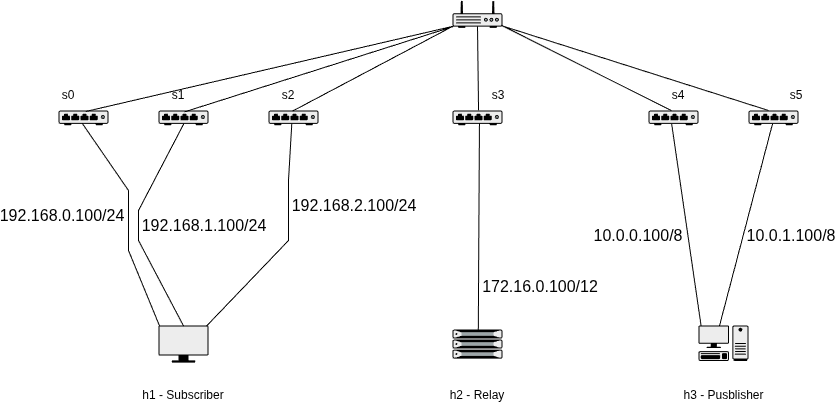
\includegraphics[width=15cm]{topoX}
\caption{A Mininetben létrehozott topológia logikai ábrázolása}
\end{figure}
 
A h1, h2, h3 jelölik a hostokat, s0-s5 jelölik a switch-eket, és r0 jelöli a routert.
h1 három interfésszel rendelkezik, egyenként csatlakozik a s0, s1 és s2 switch-ekhez, azok pedig a r0 routerhez.
Hasonlóan h2 is, csak egy interfésszel, a h3 pedig kettővel csatlakozik.

A hostok és a router között azért van szükség switch-ekre,
mert a kapcsolatok megszakítása emuláció közben problémát okoz, ha a megváltoztatott kapcsolat közvetlenül a host-okhoz csatlakozik, 
mivel az alapértelmezett átjárók alhálózatonként eltérnek, így ha egy közvetlen linket megszakítunk (amely külön alhálózaton van a többi interfészhez képest), 
akkor az alapértelmezett átjáró információja is elveszik, és a link újraépítése után nem tartozik hozzá alapértelmezett átjáró, tehát nem tesztelhető 
az az eset, amikor a link megszakítása után azt visszaállítjuk.
Így az alábbi topológián egy switch és a router közötti kapcsolat megszakításával könnyen lehet emulálni a kapcsolat 
megszakadását az alapértelmezett átjáró eltűnési problémája nélkül.

IP-alapú címzés szempontjából a hostok eltérő alhálózatokban vannak, (a h1-nek még emellett 
mindhárom interfésze eltérő alhálózatban van, hogy az alapértelmezett átjáró eltérő lehessen, ezzel pontosabban emulálva a valós környezetet).
Mindez azért is fontos, mert bár a MoQ egy alkalmazásrétegbeli (Layer 7) protokoll, a 
működéséhez elengedhetetlen a hálózati réteg (Layer 3) megfelelő működése is. A multipath viselkedés 
ugyanis IP-szinten – azaz hálózati interfészekhez és címekhez rendelt útvonalak mentén – valósul meg, 
így a tesztelés során szükséges az alsóbb rétegek kontrollált kezelése is.

A topológia kialakítása során cél volt, hogy a multipath továbbítás minden releváns esete tesztelhető legyen.
Például a h1 három interfésszel rendelkezik, hogy biztosítva legyen az, hogy nem csak két interfészen működik a multipath, azért van h3-nak is két interfésze, 
hogy meg lehessen figyelni hogy viselkedik h2 egynél több multipath kapcsolat esetén, 
vagy éppen a router és az alhálózatok is elhagyhatóak a működés szempontjából, azonban valós környezetben ezek kikerülhetetlenek. 

A munkát és a tesztelést felgyorsítva mindezt egy Python szkript segítségével automatizáltam, 
amely a Mininet API-ját használja a virtuális gépek és kapcsolatok létrehozására, konfigurálására, kezelésére, beleértve
a hostokon futtatott demonstrációs programokat és a Wireshark csomagelkapást is.
Tehát egy script futtatásával pillanatok alatt megfigyelhető a kívánt program működése.

\subsubsection{A PicoQUIC programkönyvtár}

\subparagraph{}
A fejlesztéshez elengedhetetlen a PicoQUIC alapvető ismerete, amihez megfelelő alapot képez a picoquicdemo program.
A picoquicdemo egy egyszerű példa a PicoQUIC használatára, amely bemutatja a
PicoQUIC könyvtár alapvető funkcióit és lehetőségeit, beleértve a kapcsolat
felépítését, adatátvitelt és a hibakezelést, illetve multipath funkcionalitást is kínál. 

Maga a pcioquicdemo felépítése elég egyszerű, olyan értelemben hogy ez egy darab C fájl, amely a PicoQUIC függvényeit használja, 
és a szerver, valamint a kliensek funkcióit is ellátja egyaránt. 

Sajnos pont emiatt az átláthatóságot nem feltétlen egyszerűsíti meg, de összességében kiderült, hogy két dolog szükséges a multipath működéshez.

Egyrészt a kezdeti multipath negotiation (egyeztetés) – ami arra szolgál, hogy a két fél közötti első
kapcsolat felépítésekor megegyezzenek az összes többi transzport paraméter mellett abban is, 
hogy mind a két fél támogatja-e a többutas kapcsolatot; másrészt az "extra" útvonalak tényleges kiépítése.

Ezek közül az utóbbit megvalósító kódrészletek könnyen elkülöníthetőek a kód többi részétől, mivel ezen a 
téren a program sok fajta opciót biztosít, amelyek közül a legegyszerűbb eshetőség az alapszintű 
multipath, amikor több interfész használatával több útvonalat alakítunk ki, amelyeket a PicoQUIC könyvtár automatikusan kezel.

Jelenlegi munka szempontjából ez az egyszerű multipath a leginkább releváns,
mivel amíg az nem működik megfelelően, addig a komplexebb multipath forgatókönyvek nem is igazán tesztelhetők/használhatók.
Az ezt ellátó kódrészlet a picoquicdemo-ban jól elkülönül, így jó alapot biztosított a LibQuicR könyvtárbeli implementációhoz.

\subsubsection{Egyéb következtetések a PicoQUIC kapcsán}

A Wireshark használata során érdekes kérdés merült fel a multipath PicoQUIC implementálásával kapcsolatban,
mégpedig, hogy nem feltétlenül kezeli a kapcsolat útvonalait az IETF QUIC Multipath draftja szerint, mivel adott útvonal kapcsán útvonal szakadás 
esetén nem láttunk PATH ABANDON üzenetet, ami arra szolgálna, hogy egy már nem működő útvonalat inaktívvá nyilvánítson mind a két fél számára.
Azonban olyan érdekes jelenség is előfordult, hogy A és B útvonal esetében A útvonal megszakítása után B útvonalon ment tovább az adatátvitel,
de ha A útvonal újra aktívvá vált, akkor nem használta újra azt, és ezután B útvonal megszakítása után sem váltott vissza A útvonalra. Ami ezt még inkább érdekessé 
teszi, az az, hogy B útvonalat újra aktiválva az adatátvitel folytatódott. Tehát a PicoQUIC multipath implementációja nem feltétlenül
kezel minden esetet a draft szerint, de ez nem feltétlenül jelent problémát a jelenlegi fejlesztési szakaszban, 
mivel a protokoll még nem végleges, és ez a viselkedés egyben kijelölhet egy lehetséges irányt a projekt további bővítésére vagy finomhangolására.

\subsubsection{Működés elemzésének módjai}

\subparagraph{}

A PicoQUIC rengeteg funkciót és metrikát biztosít a működés elemzésére, 
első sorban a qlog fájlok generálása lenne a bevett módszer, és
a protokoll alapszintű működésének megértése szempontjából valóban hasznos 
a qlog, de nem minden esetben elegendő, mivel a QUIC protokoll
sokféle eseményt és metrikát generál, amelyek közül sok nem feltétlenül releváns a 
multipath működés szempontjából és maga a multipath is megnehezíti mivel a qlog események 
elemézésére használatos qvis program\cite{qvis} – ami egy webes alkalmazás, a qlog 
fájlok vizualizálására – nem képes könnyen és átláthatóan megjeleníteni a multipath 
eseményeket, mivel azok könnyen eltorzítják a két oldal kapcsolatának 
szinkronizációját, így ezzel nem lehet megfelelően elemezni a kapcsolatokat.

\paragraph{}
A qlog fájlok elemzésénél sokkal hasznosabb a Wireshark program, mivel
a QUIC protokollt is támogatja.
Azonban ez olyan kihívást állít a qlog-gal szemben, hogy míg a 
qlog fájlokat a program maga generálja, tehát a titkosítást ki tudja kerülni, 
addig a Wireshark magukat a hálózati interfészen megjelenő csomagokat rögzíti, 
így a QUIC csomagok titkosítása megnehezítette a folyamatot, főleg a multipath 
miatt, mivel a másodlagos útvonalon küldött és fogadott csomagokat a Wireshark 
nem tudja hozzákötni automatikusan az első útvonal interfészén létrejött kapcsolat titkosított csomagjaihoz.

A PicoQUIC beépítetten támogatja a SSL keylog fájlok generálását a "SSLKEYLOGFILE" környezeti változó 
beállításával, ami segítségével fel lehet oldani a QUIC által használt TLS titkosítást,
így a Wireshark képes dekódolni a csomagokat, és megjeleníteni azok 
tartalmát (legalábbis a kapcsolat kezeléséért felelős QUIC réteg szempontjából).

Ez a megoldás lehetővé teszi, hogy a Wireshark segítségével generált 
pcapng fájlokat átkonvertáljuk dekódolt formátumra az alábbi paranccsal:
\begin{verbatim}
  editcap --inject-secrets tls,<keylog_file> <input_pcap_file> 
    <output_pcap_file>
\end{verbatim}
Ez a parancs a Wireshark által generált TLS titkosítást használó QUIC 
csomagokat tartalmazó pcapng fájlokat dekódolja, a keylog fájl segítségével, így azok bármilyen kontextusban, a keylog fájl nélkül megtekinthetőek
és elemezhetőek.


\subsubsection{LibQuicR felépítése és átalakítása}
\paragraph{}

A LibQuicR könyvtár egy összetettebb kódbázisú program mint a picoquicdemo, mivel amíg az utóbbi egy darab C fájl, 
ami direkt használja a PicoQUIC könyvtárat demonstrációs célokra,
addig a LibQuicR sokkal komplexebb struktúrával rendelkezik, amelyben a PicoQUIC könyvtár sokkal kevésbé közvetlenül van jelen.
Ennek ellenére pont azért, mert egy jelentősen nagyobb struktúráról van szó, szükségszerűen sokkal 
jobban elkülönülnek a különböző funkciók, így a PicoQUIC API-ját használó kódrészletek is.

A multipath működés támogatásához három fő funkció került implementálásra a LibQuicR könyvtárban. 
Egyrészt bővítésre került a parancssori felhasználói felület (CLI), amely új, multipath-specifikus 
argumentumokat fogad. Másrészt megvalósításra került a multipath negotiation folyamata, valamint a 
másodlagos hálózati útvonalak kiépítésének logikája is.

Ebből a második és harmadik megegyezik a korábban PicoQUIC-nél említettekkel, mivel ezek elengedhetetlenek a multipath működéshez,
de ahhoz, hogy ezt érdemben lehessen használni is, szükséges volt a CLI argumentumok kiegészítése is.
Ezt a picoquicdemo-ban használatos argumentumokhoz hasonlóan 
valósítottam meg, mivel ha már PicoQUIC-re alapoz a LibQuicR, és maga a fejlesztésem pedig annak a 
multipath demonstrálására szolgáló demó programjára alapoz, akkor a CLI argumentumoknak hasonló megválasztása egy logikus lépés.

Relay esetén ez a CLI argumentumok kiegészítése csak egy extra argumentumot jelentett:
\begin{verbatim}
  -m, --multipath
\end{verbatim}
Ez egy szimpla kapcsoló (nem fogad extra paramétert), amely oly módon engedélyezi a multipath támogatást, 
hogy amikor létrejön a relay objektum QUIC transzportért felelős része,
akkor azt úgy inicializálja, hogy egy bejövő kapcsolat esetén a transzport paraméterek 
egyeztetésénél a saját paraméterei között szerepeljen a multipath támogatás is.

Végponti kapcsolat esetén ez két kiegészítést jelentett:
\begin{itemize}
  \item \texttt{-m, --multipath}
  \item \texttt{-a ``\ldots'', --alt\_ifaces ``\ldots''}
\end{itemize}

Itt természetesen a multipath kapcsoló ugyanúgy működik mint a relay esetén,
de emellett szükséges volt egy új argumentum is, amely lehetővé teszi a felhasználó számára, hogy megadja a másodlagos interfészeket,
amelyeken a multipath harmadik szükséges elemét, a másodlagos útvonalakat kiépíti. Ehhez szüksége van paraméterekre, amelyek a másodlagos interfészeket
tartalmazzák, itt is a picoquicdemo-val azonos formátumot használtam, tehát a következő formátumot várja:
\begin{verbatim}
  -a "<IP-cím>/<interfész száma>,<IP-cím>/<interfész száma>,..."
\end{verbatim}
Például a h1 host esetén ez az alábbi módon néz ki: "192.168.1.100/3,192.168.2.100/4". Látható, hogy az alapértelmezett IP-címre nincs 
szüksége, mert azon már elkezdődött a kapcsolat, és csak azokat az interfészeket kell megadni, amelyeken a másodlagos útvonalakat kiépíti. 

Az eltérés a relay és a végponti kapcsolat között abban rejlik, hogy míg a relay fogadja a bejövő kapcsolatokat, addig a végponti kapcsolat esetén önállóan,
a kapcsolat létrejötte után küld PATH CHALLENGE üzeneteket a másodlagos interfészeken, 
hogy azok is elérhetővé váljanak a kapcsolat számára (amennyiben a multipath negotiation sikeresen megtörtént).
Relay esetén több interfész használatát nem implementálja jelenleg a munkám.

\paragraph{}

A multipath negotiation megvalósulásához ki kellett egészíteni a LibQuicR-ben
használt adatstruktúrákat, hogy eljussanak a multipath és az interfész információk
arra a szintre, ahol a PicoQUIC könyvtár API-ját használja a program, valamint 
a PicoQUIC transzport objektum konstruktorát 
kellett kiegészíteni, és a transzport paraméterek inicializálásakor a multipath paraméter mellett az 
  \texttt{initial\_max\_path\_id}
változót kellett beállítani, hogy kapcsolat létrehozása után tudjon kezelni több útvonalat is.

\paragraph{}

A többi útvonal kiépítése gyakorlatilag megegyező módon működik, mint a picoquicdemo esetén. A PicoQUIC 
  \texttt{packet\_loop\_v3()}
függvénye minden egyes csomag feldolgozása után meghív egy callback függvényt, amely a LibQuicR könyvtárban van 
implementálva, és ebben történik meg – ha minden körülmény adott, tehát kliensről van szó, 
multipath engedélyezett, és addig a pontig még nem volt új útvonal próbálva – hogy a másodlagos interfészeken PATH CHALLENGE üzeneteket küldjön.
Ebben a callback függvényben történik egy segédfüggvény segítségével a másodlagos interfészeket tartalmazó sztring feldolgozása is, amely logikailag
ugyancsak azonos módon működik mint a picoquicdemo esetén.


\subsubsection{Funkcionális tesztelés}
\paragraph{}

Módosításaim eredményeként a bemutatott környezetben működik a többutas adatávitel, 
amely a másodlagos interfészeken keresztül adatokat küldeni és fogadni, továbbá valamely útvonal megszakadása esetén
minimális késleltetéssel képes a másodlagos interfészen folytatni az adatátvitelt.
Maga az adatátvitel időbélyegek másodpercenkénti küldését jelenti, ami egy beépített módja a LibQuicR demó programjának.

A következő ábrák a bmon program kimenetét mutatják a h1 hoston, amely subscriber üzemmódban fut és három interfészen, interfészenként
külön alhálózaton kommunikál a h2 hosttal egy rotueren keresztül, amely relay-ként üzemel.

\begin{figure}[h]
  \centering
    \hspace*{-1.5cm}% vagy amennyivel szükséges
    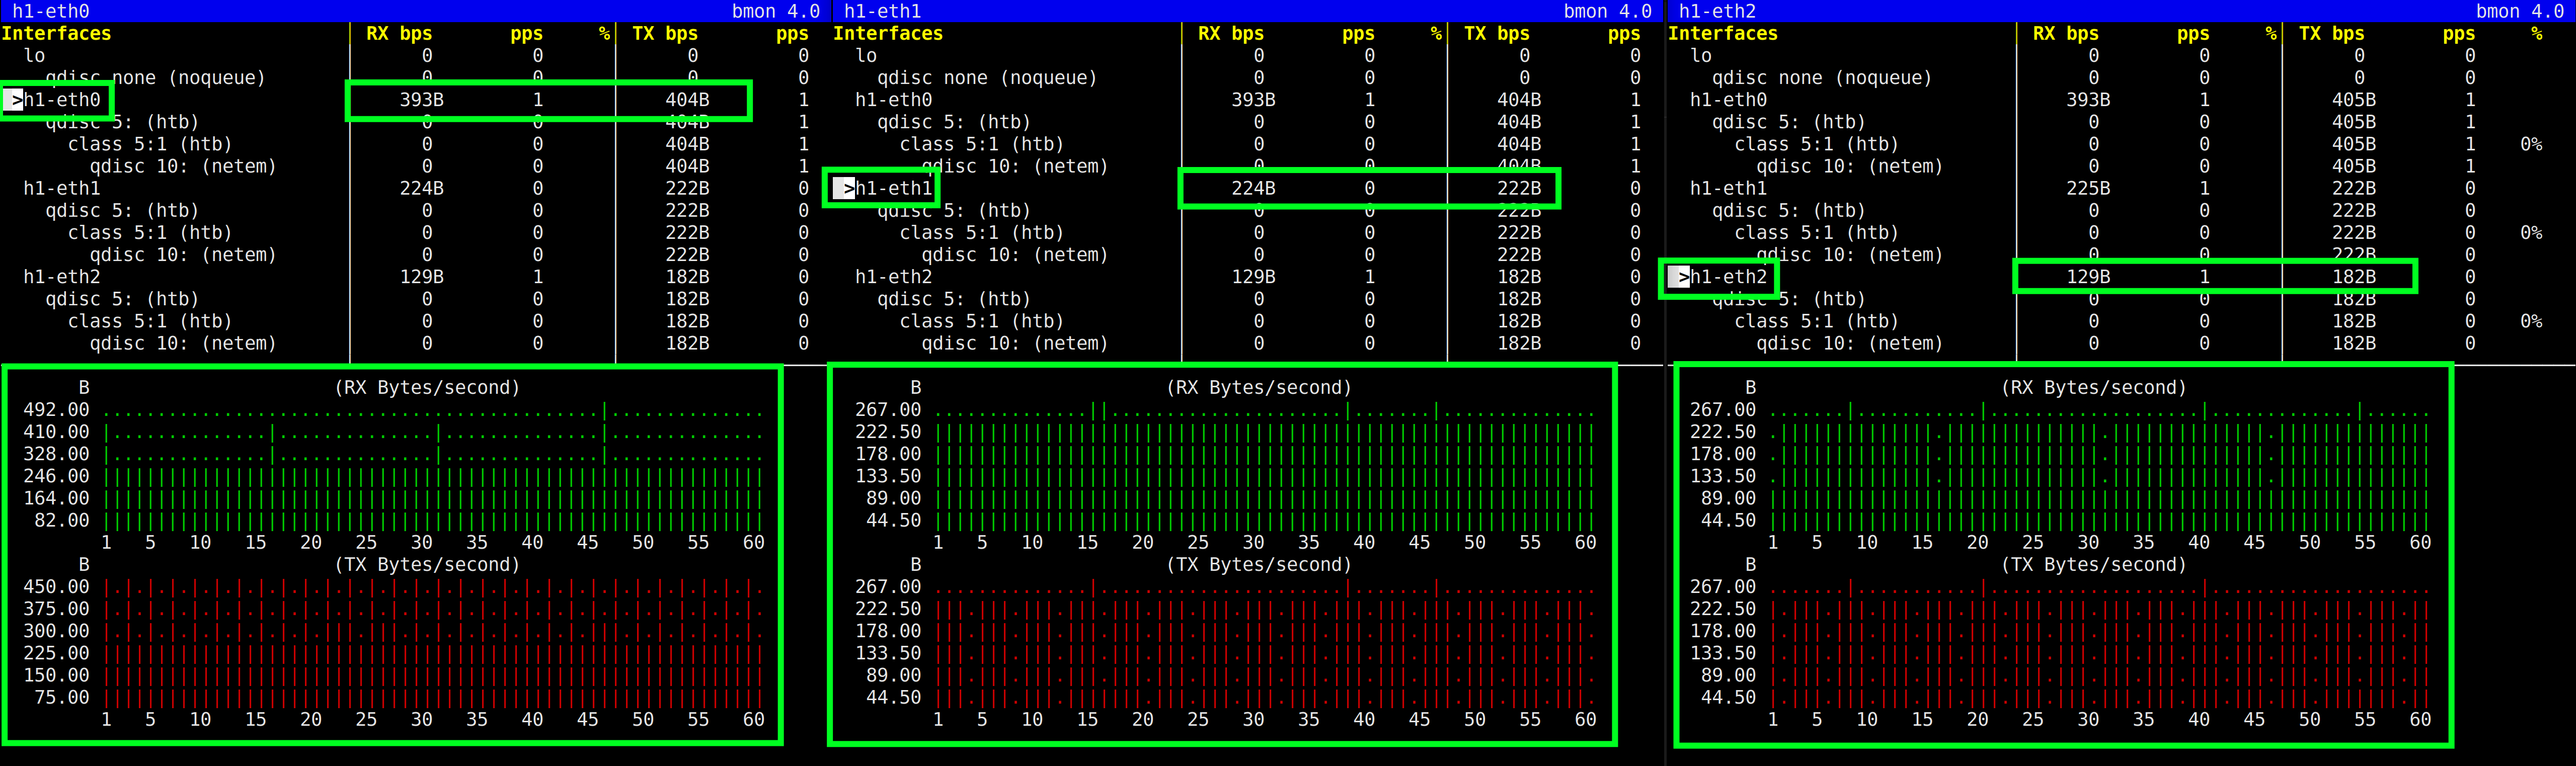
\includegraphics[width=18cm]{bmon11}
\caption{Interfész aktivitás 3 aktív útvonallal, sorrendben 0, 1, és 2-es indexű interfészek}
\end{figure}

2. ábrán látható, hogy 3 aktív interfészen keresztül van folyamatos adatátvitel, majd a 3. ábrán 
már látható, hogy a nullás indexű interfészen nem folyik adat, mivel itt az ahhoz kapcsolódó switch és a router közötti kapcsolatot megszakítottam.
Ezért a másodlagos interfészeken keresztül folytatódik az adatátvitel. Ezek nem csak azt bizonyítják, hogy a multipath 
implementáció kezeli a kapcsolatszakadást, de azt is, hogy akár 3 interfészt is tud hasznosítani.


\begin{figure}[h]
  \centering
    \hspace*{-1.5cm}% vagy amennyivel szükséges
    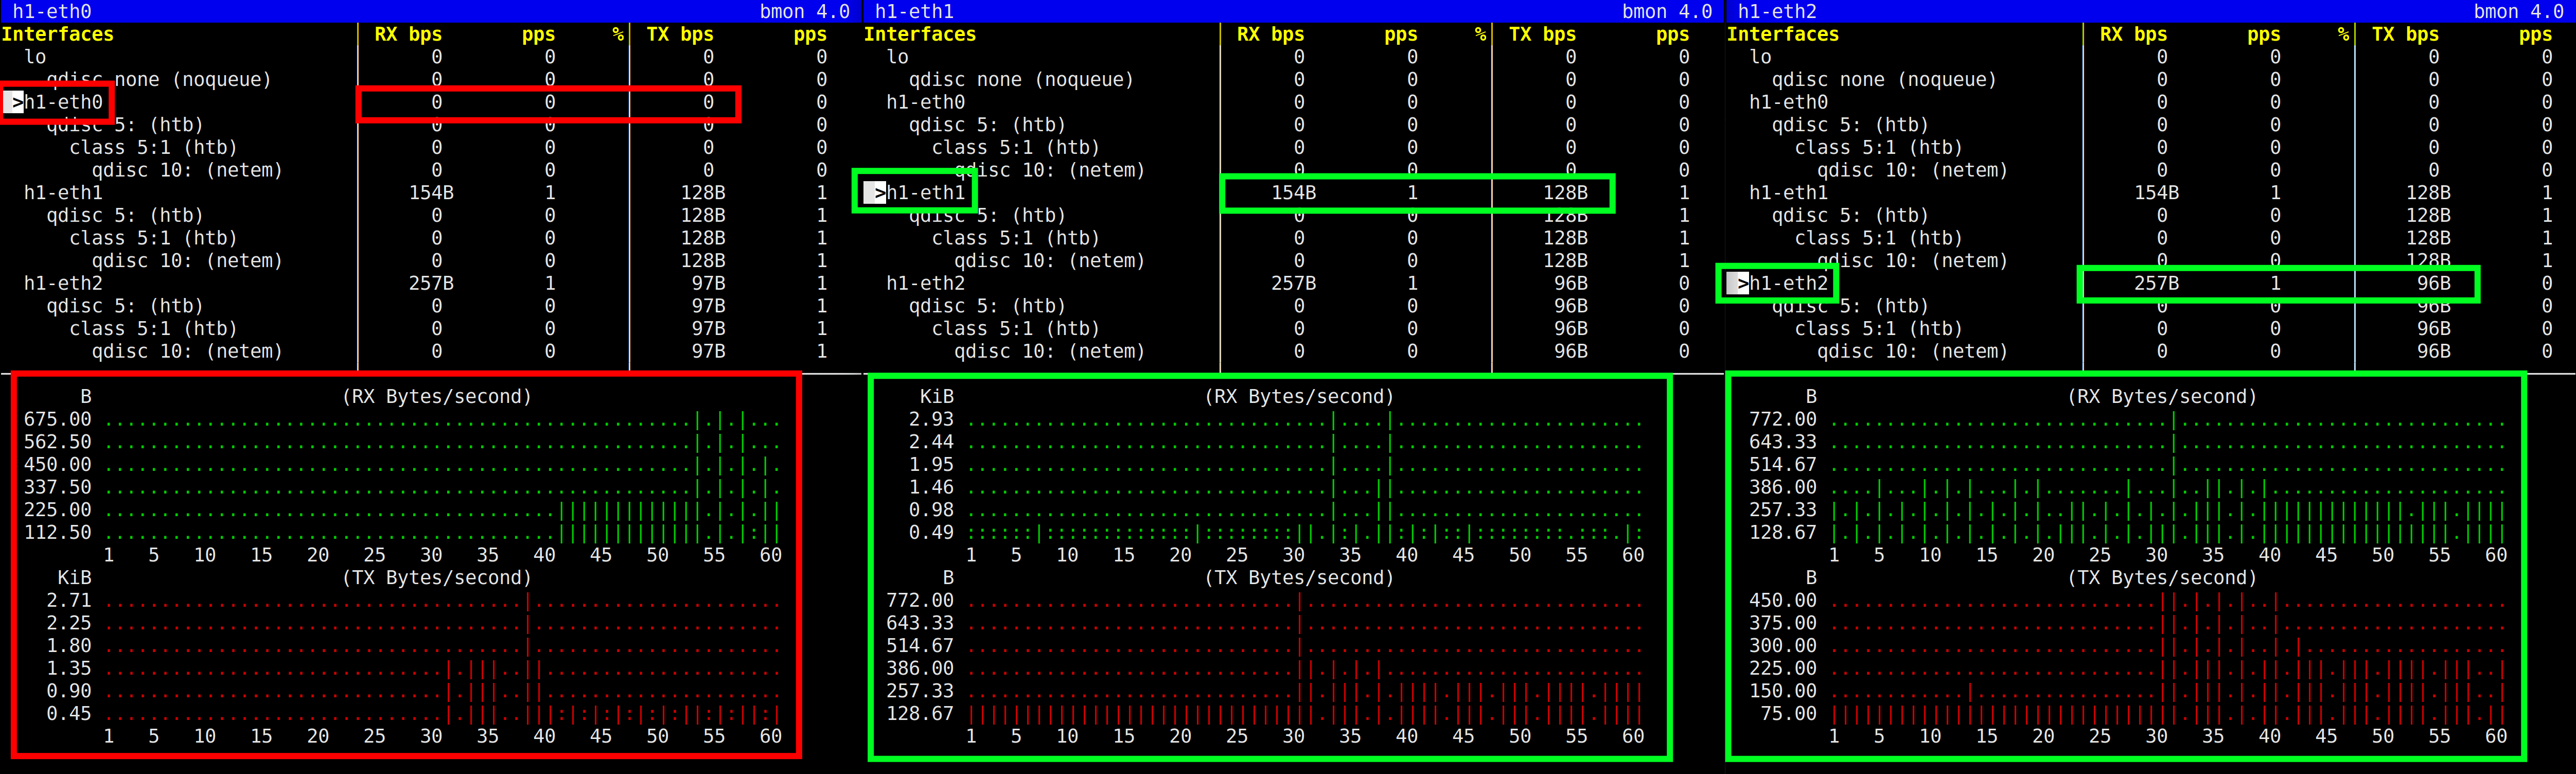
\includegraphics[width=18cm]{bmon22}
\caption{Interfész aktivitás 2 aktív útvonallal, sorrendben 0, 1, és 2-es indexű interfészek}
\end{figure}

Majd pedig a 4. ábrán látható, hogy az egyes indexű interfészen is leállt az adatátvitel (ugyancsak 
kapcsolatszakadás miatt), de a kettes indexű interfészen továbbra is fennmarad az adatátvitelt.

\begin{figure}[h]
  \centering
    \hspace*{-1.5cm}% vagy amennyivel szükséges
    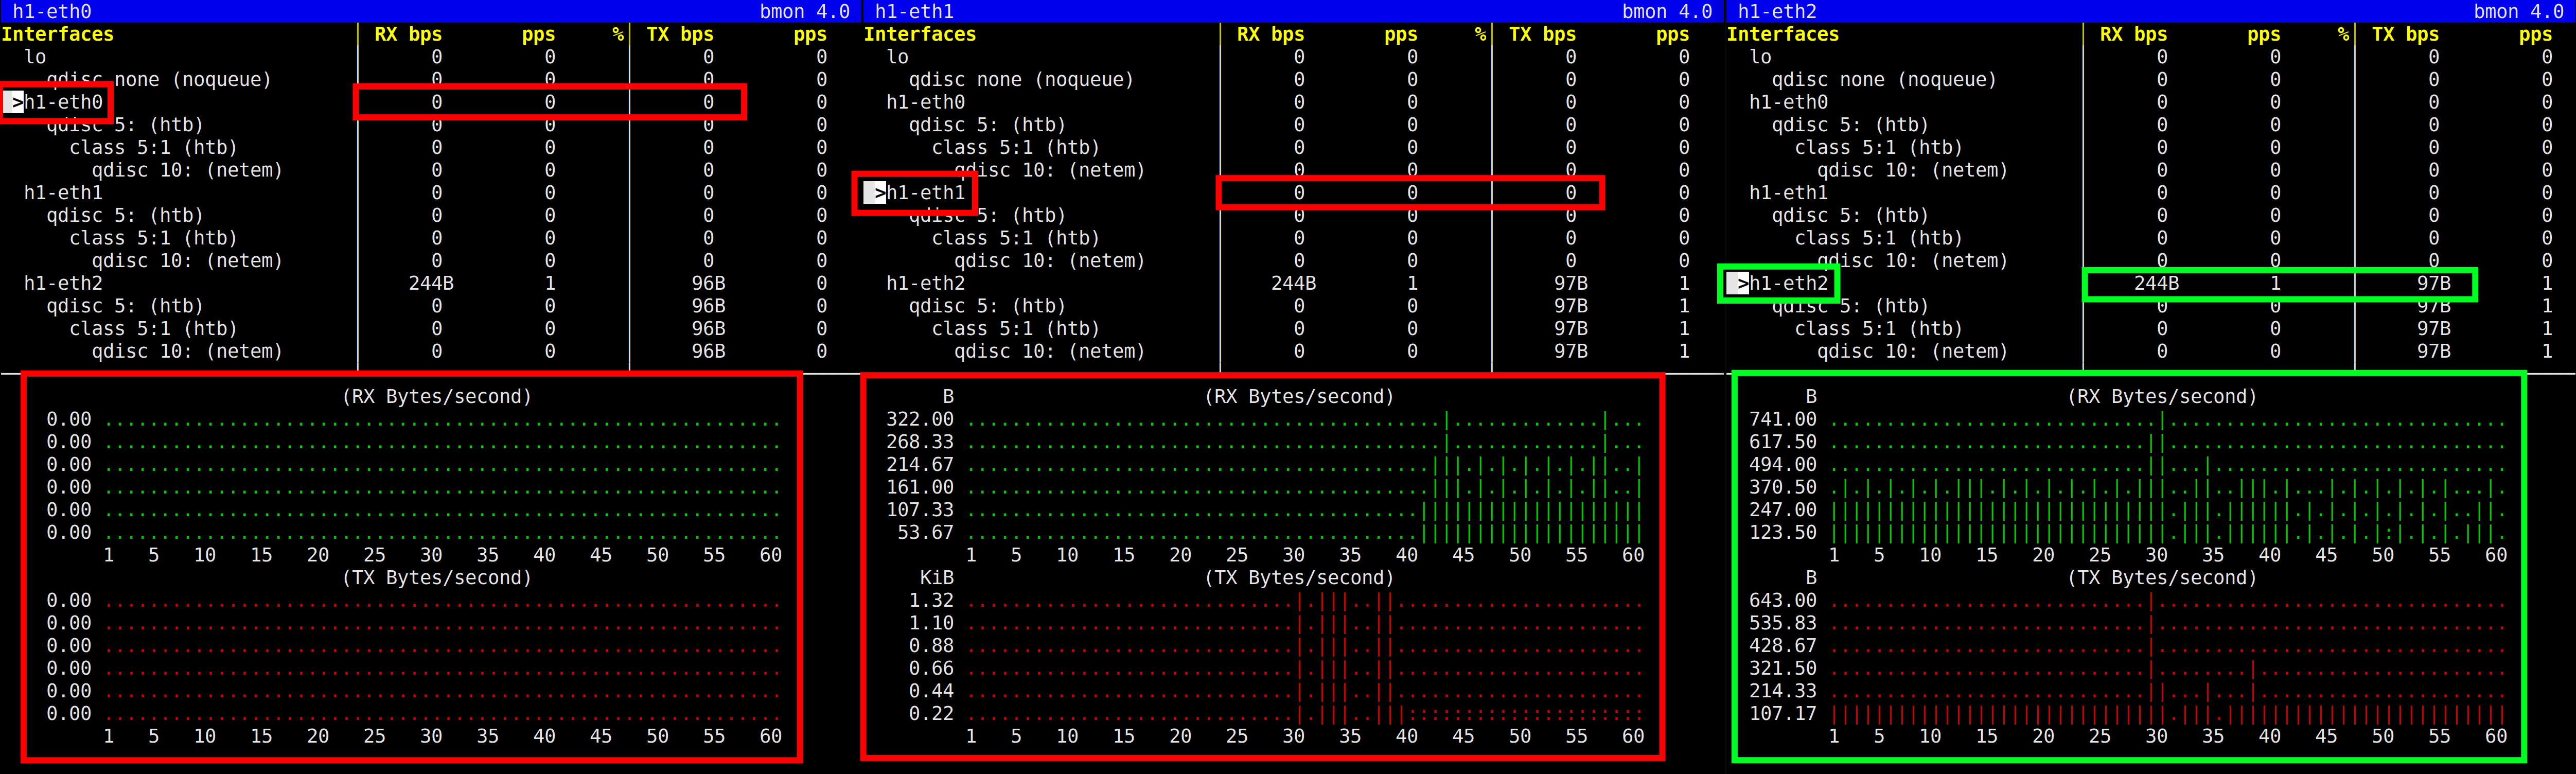
\includegraphics[width=18cm]{bmon33}
\caption{Interfész aktivitás 1 aktív útvonallal, sorrendben 0, 1, és 2-es indexű interfészek}
\end{figure}

Fontos megjegyezni, hogy a relay minimális kódmódosítással képes kezelni valamennyi 
releváns kapcsolódási szituációt. Ennek megfelelően működőképes akkor is, ha a subscriber és a 
publisher egyaránt egyetlen hálózati interfészen keresztül csatlakozik, ha csak az egyik 
fél – például a subscriber vagy a publisher – rendelkezik több interfésszel, illetve abban 
az esetben is, ha mindkét végpont több interfészen keresztül kapcsolódik a hálózathoz.


Illetve érdekes azt is megjegyezni, hogy a korábban említett 
  \texttt{initial\_max\_path\_id}
változó a kódban 2-re van állítva, ha multipath környezetben indul el a program,
de ez nem korlátozza le kapcsolatonként két interfész használatára sem a relayt, sem pedig a 
subscribert vagy a publishert, mint látható a 2. ábrán, ahol 3 interfész van aktívan használva.

\subsection{Összefoglalás}
\label{sec:osszefoglalas}

\subsubsection{Féléves feladat összefoglalása}
\paragraph{}

Féléves feladatom a QUIC feletti médiaátvitelt megvalósító LibQuicR könyvtárban egy kezdetleges multipath támogatás 
implementálása volt, valamint ehhez kapcsolódóan egy demonstrációs környezet kialakítása és a megvalósítás 
működésének értékelése. A munka során az alábbi eredményeket értem el:

\begin{itemize}
\item A LibQuicR könyvtárban a multipath működést kezdetlegesen implementáltam, 
amely megalapozhatja a jövőbeni, fejlettebb multipath támogatást a projektben. Implementációm GitHub repository-ja: 
\href{https://github.com/Schweitzee/libquicr/tree/multipath}{github.com/Schweitzee/libquicr (multipath branch)}
\item A fejlesztést dokumentáltam, a megvalósítást letisztáztam és előkészítettem 
GitHub-on történő közzétételre pull request formájában az eredeti projekthez.
\item SSL keylog fájl generálásának lehetőségét beépítettem a LibQuicR könyvtár 
általam módosított verziójába, ez segíti a protokoll működésének nyomon követését 
és az elemzést például Wireshark eszközzel. Elvégzett módosítások: 
\href{https://github.com/Schweitzee/libquicr/tree/ssl-keylog}{github.com/Schweitzee/libquicr (ssl-keylog branch)}
\item A Mininet program segítségével egy demonstrációs környezetet alakítottam ki, 
amelyben a megvalósítás különböző hálózati szcenáriókban is kipróbálható.
\end{itemize}

\subsubsection{Továbbfejlesztési lehetőségek}
\paragraph{}
Ez az implementáció az első ilyen jellegű próbálkozás a Media over QUIC (MoQ) architektúrában, és bár 
jelenleg csupán kezdetleges multipath funkcionalitást nyújt, már most jól látható, hogy számos továbbfejlesztési 
lehetőséget kínál, amelyek megvalósításához a félév során elvégzett munka szilárd kiindulási alapot jelent. 

A projekt lehetséges folytatási irányai közé tartozik például a relay oldali fejlesztések kibővítése oly 
módon, hogy az ne csupán egyetlen, hanem több interfészt is képes legyen aktívan használni a továbbítás 
során. 

Emellett további multipath képességek is implementálhatók, amelyek a PicoQUIC picoquicdemo 
programjában már elérhetők, de ebben az implementációban még nem kerültek alkalmazásra. Ilyen lehetőség 
például a kapcsolati azonosítók dinamikus megújítása, vagy a NAT rebinding kezelése. Utóbbi alatt 
azt értjük, hogy a hálózati címfordító (NAT) eszköz egy új külső IP-cím és port párost rendel a 
klienshez – például újracsatlakozás esetén –, amit a protokollnak megfelelően le kell tudni követni. 
Szintén megvalósítható az azonos IP-címről, de eltérő porttal indított új útvonalak kezelése, illetve 
annak a lehetősége is, hogy a kapcsolat teljes egészében átmigráljon egy másodlagos interfészre, ha 
például az elsődleges hálózati kapcsolat megszakad vagy instabillá válik. 

Ezen felül érdemes megvizsgálni a 
multipath továbbítás alkalmazhatóságát relay-ek közötti kapcsolatok esetén is, hiszen ez további 
redundanciát és rugalmasságot biztosíthat a rendszer egészében. 

Végül egy hosszabb távú fejlesztési 
irány lehet egy olyan demonstrációs program készítése, amely valós médiatartalmakat – például élő 
videó streamet – továbbít multipath használatával, ezzel lehetőséget nyújtva a gyakorlati előnyök 
részletesebb értékelésére és bemutatására.

\newpage
 
%==================================================================
\section{Irodalom, és csatlakozó dokumentumok jegyzéke}
\label{sec:irod-es-csatl}

\begin{thebibliography}{9}
\label{sec:tanulm-irod-jegyz}

\bibitem{live_stats} Douglas Karr, \emph{Live Streaming Trends and Statistics (2024)}, (Accessed: 2024-05-12)\\ 
\url{https://martech.zone/live-streaming-trends-statistics/}

\bibitem{quic} J. Iyengar and M. Thomson.
\newblock QUIC: A UDP-Based Multiplexed and Secure Transport.
\newblock RFC 9000, IETF, May 2021.\\
\url{https://www.rfc-editor.org/rfc/rfc9000}

\bibitem{mp_quic} QUIC Working Group, \emph{Multipath Extension for QUIC, draft-ietf-quic-multipath-14, 2025. apr. 24.}\\
\url{https://datatracker.ietf.org/doc/draft-ietf-quic-multipath/14/}

\bibitem{pico_git} Christian Huitema / Private Octopus Inc., \emph{PicoQUIC}, [GitHub repository], (Accessed: 2024-05-12)\\
 \url{https://github.com/private-octopus/picoquic}

\bibitem{moq_draft} IETF, \emph{Media over QUIC Transport, 2025. apr. 28.}, \url{https://datatracker.ietf.org/doc/draft-ietf-moq-transport/11/}

\bibitem{mininet}
Bob Lantz, Brandon Heller, and Nick McKeown.
\newblock A network in a laptop: rapid prototyping for software-defined networks.
\newblock In \emph{Proceedings of the 9th ACM SIGCOMM Workshop on Hot Topics in Networks (Hotnets-IX)}, pages 19--24, Monterey, California, 2010.
\newblock Association for Computing Machinery. \url{https://doi.org/10.1145/1868447.1868466}.

\bibitem{libquicr} Quicr, \emph{LibQuicR}, [GitHub repository], (Accessed: 2024-05-12)\\
 \url{https://github.com/Quicr/libquicr}

\bibitem{qlog}Robin Marx.
\newblock qlog: A standardized schema for logging and visualizing QUIC events. (Accessed: 2024-05-12)\\
\url{https://github.com/quiclog/qlog}

\bibitem{qvis}Robin Marx.
\newblock qvis: A web-based tool for visualizing qlog files. (Accessed: 2024-05-12)\\
\url{https://qvis.quictools.info}

\end{thebibliography}

%==================================================================
\subsection{A csatlakozó dokumentumok jegyzéke}
\label{sec:csat-irod}
\paragraph{}
Saját multipath implementációm GitHub repository-ja: \url{https://github.com/Schweitzee/libquicr/tree/multipath}

\paragraph{}
SSL keylog fájl generálásához szükséges módosítások: \url{https://github.com/Schweitzee/libquicr/tree/ssl-keylog}

\end{document} 

%%% Local Variables: 
%%% mode: latex 
%%% TeX-master: t 
%%% End:

